% Beamer summary for EIC DIS analysis (campaign 25.12.0)
\documentclass[aspectratio=169]{beamer}
\usetheme{Madrid}
\usecolortheme{dolphin}
\usepackage{graphicx}
\usepackage{amsmath}
\usepackage{physics}
\usepackage{siunitx}

\title{EIC Diff . DIS Analysis Summary}
\subtitle{Campaign 25.12.0 (126K events)}
\author{Hadi Hashamipour\\}
\date{\today}

\begin{document}

\begin{frame}
  \titlepage
\end{frame}

\begin{frame}{Dataset and Scope}
  \begin{itemize}
    \item Campaign: \textbf{25.12.0}
    \item Statistics: \textbf{126K events} (processed)
    \item Inclusive DIS kinematics (EM/DA/Sigma), diffractive variables (|t|, $x_L$)
  \end{itemize}
\end{frame}

\begin{frame}{Key Equations}
  \begin{align*}
    Q^2 &= -q^2, \quad q = k - k' \\
    x_{Bj} &= \frac{Q^2}{2 p \cdot q} \\
    y &= \frac{p \cdot q}{p \cdot k} \\
    W^2 &= (p + q)^2 \\
    |t| &= |(p - p')^2|
  \end{align*}
\end{frame}

\begin{frame}{Inclusive Kinematics: Distributions}
  \begin{columns}
    \column{0.35\textwidth}
    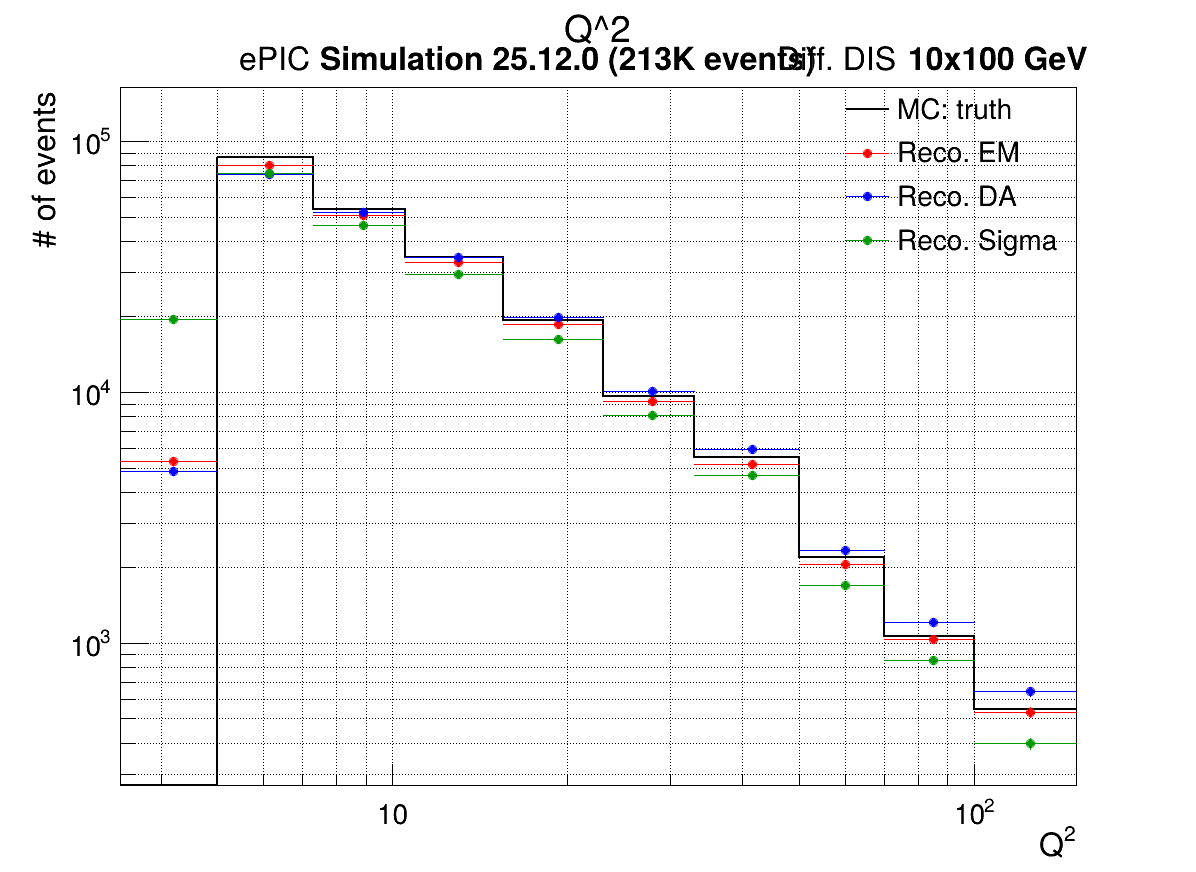
\includegraphics[width=\linewidth]{../figs/inclusive/histos/q2_methods_hist.png}
    \vspace{0.2cm}
    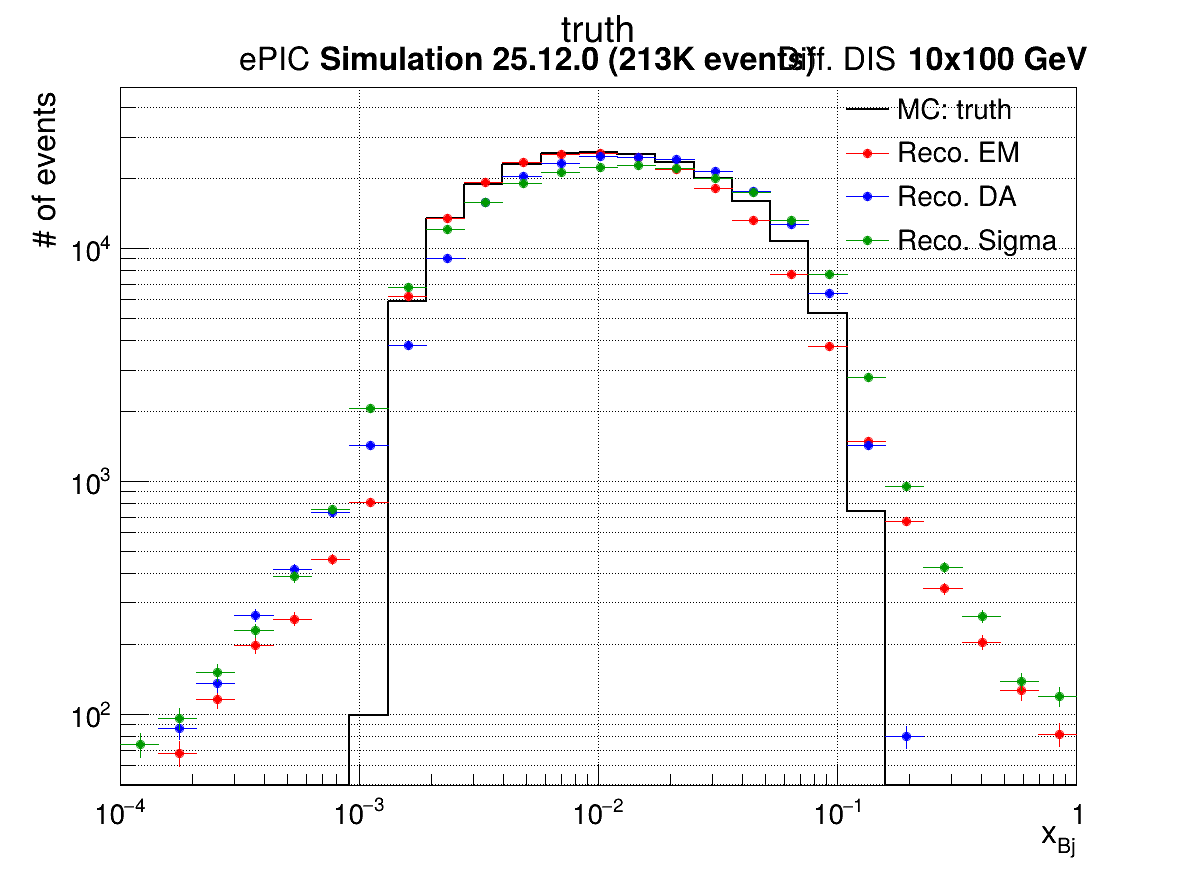
\includegraphics[width=\linewidth]{../figs/inclusive/histos/xbj_methods_hist.png}
    \column{0.35\textwidth}
    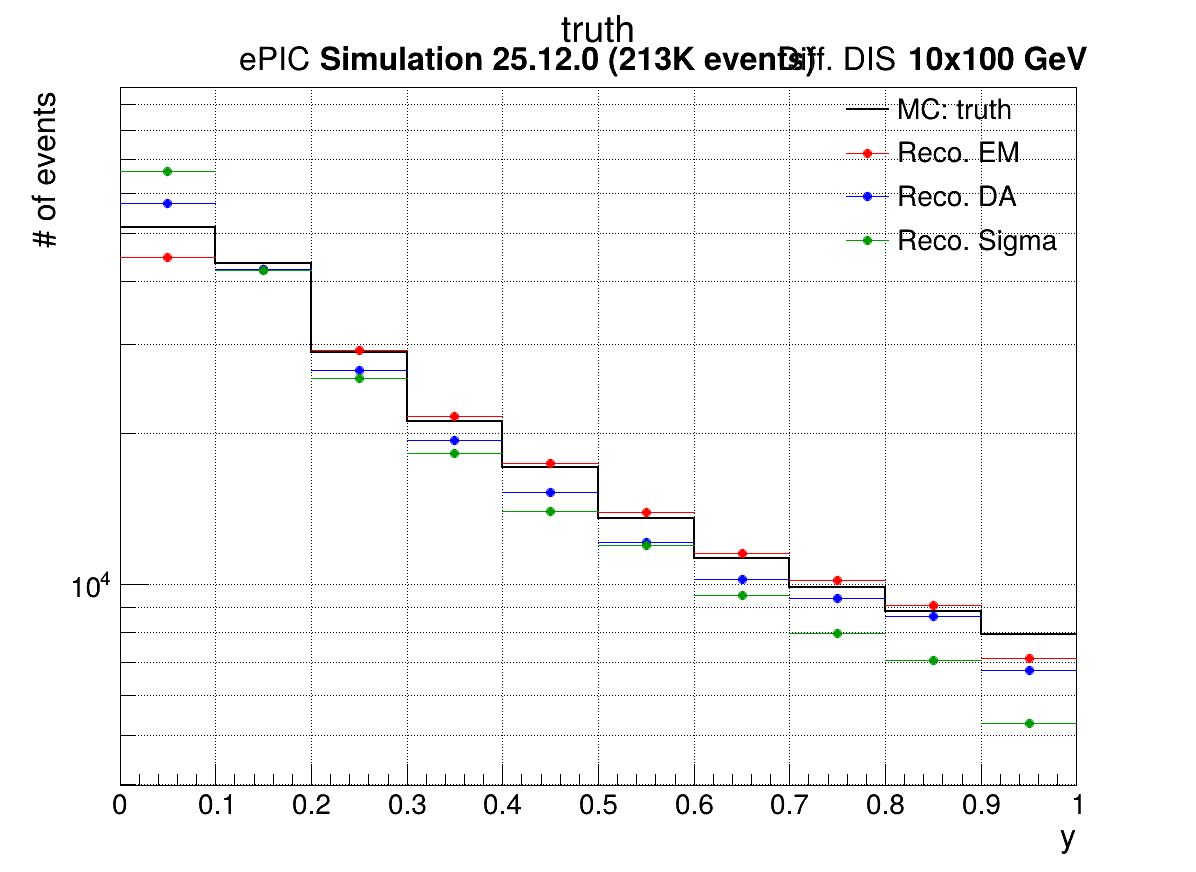
\includegraphics[width=\linewidth]{../figs/inclusive/histos/y_methods_hist.png}
    \vspace{0.2cm}
    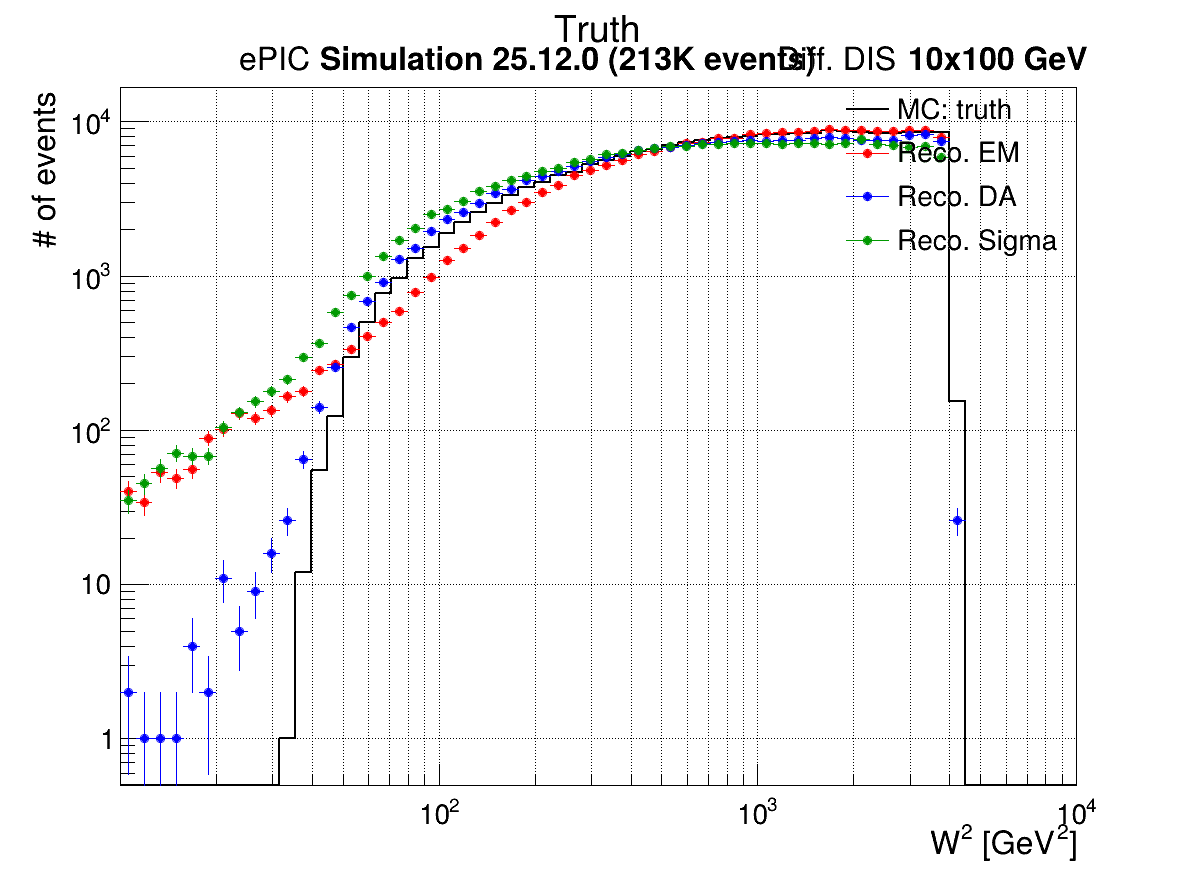
\includegraphics[width=\linewidth]{../figs/inclusive/histos/w2_methods_hist.png}
  \end{columns}
\end{frame}

\begin{frame}{Event Density in $x_{Bj}$--$Q^2$}
  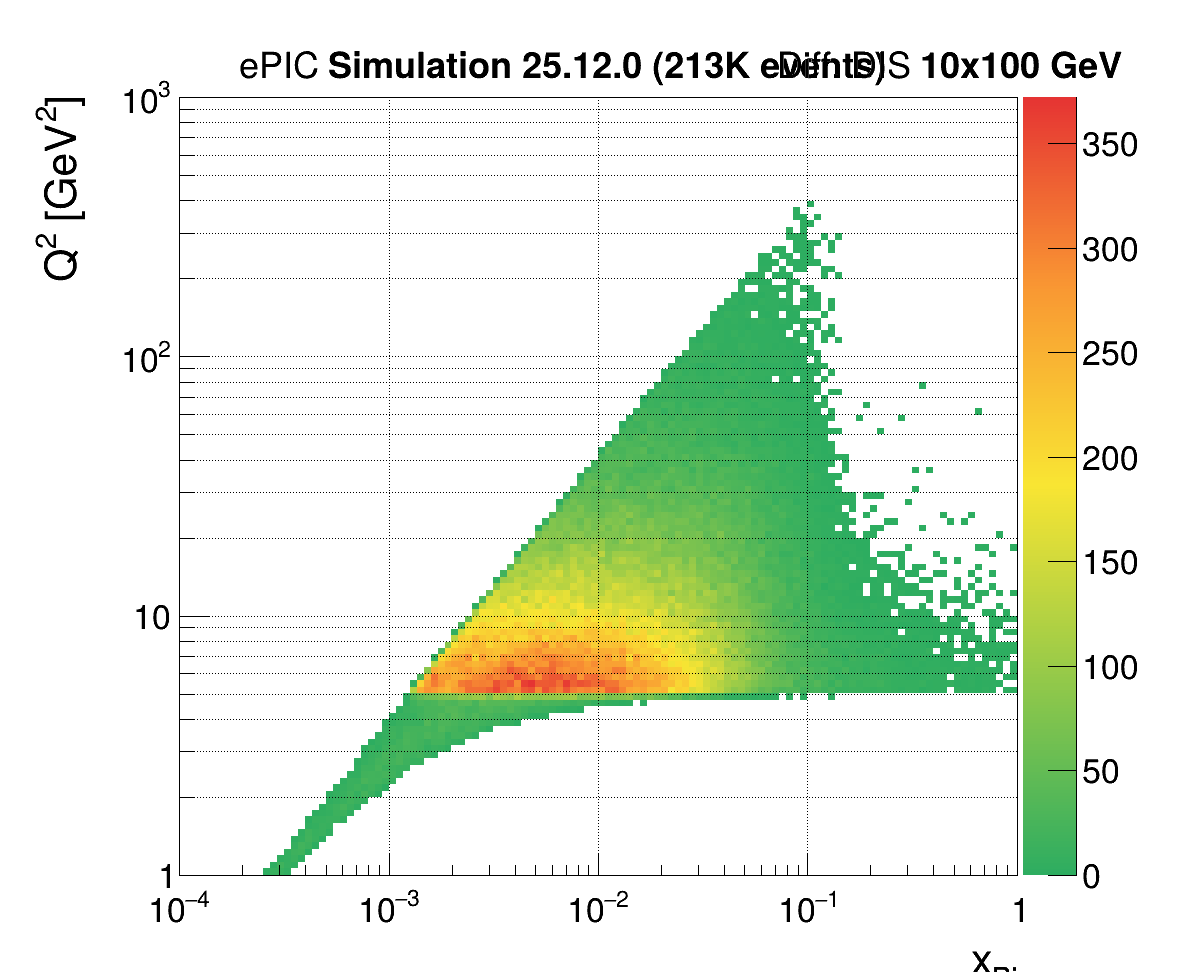
\includegraphics[width=0.6\linewidth]{../figs/inclusive/histos/xbj_q2_density.png}
\end{frame}

\begin{frame}{Inclusive Correlations (Unbinned)}
  \begin{columns}
    \column{0.25\textwidth}
    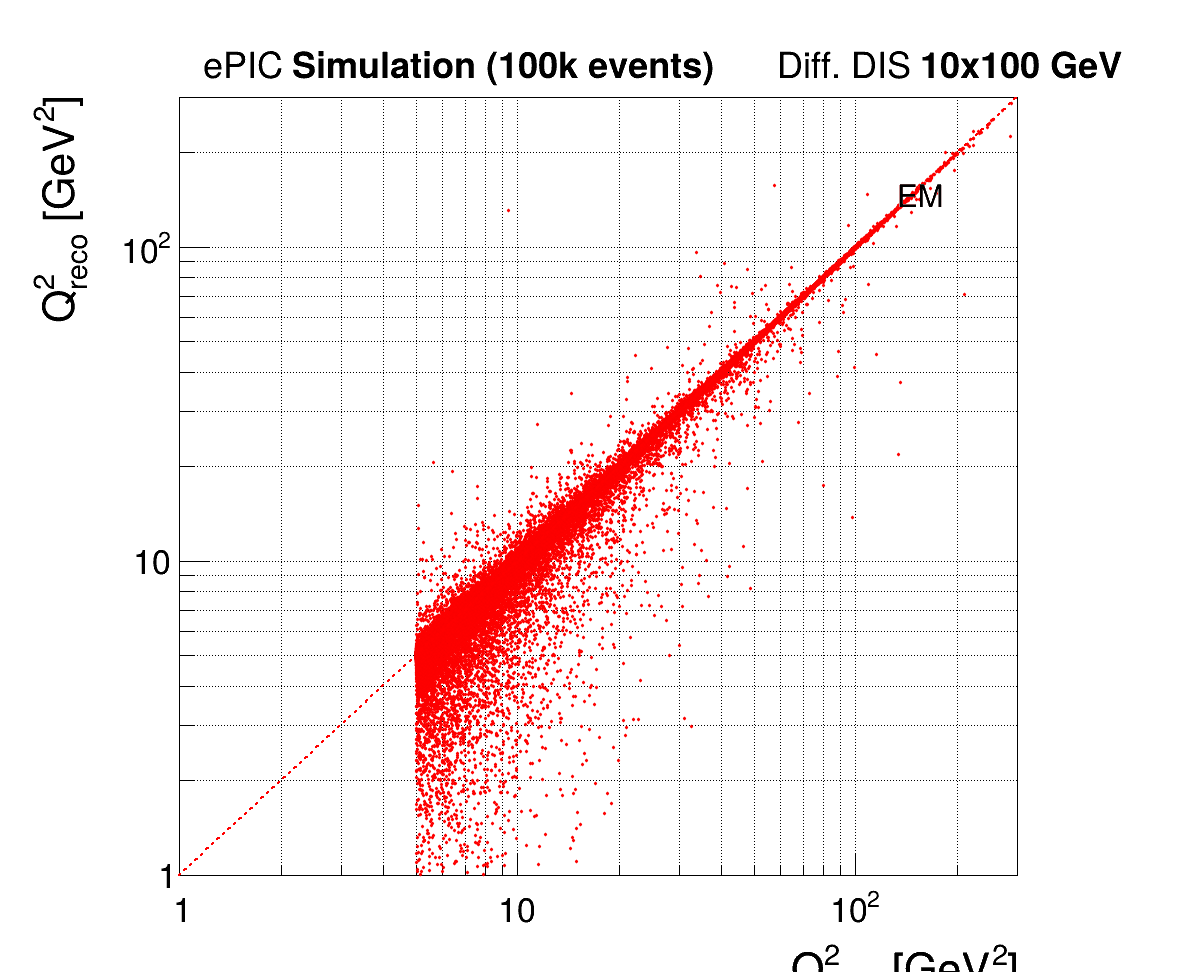
\includegraphics[width=\linewidth]{../figs/inclusive/histos/q2_corr_unbinned_em.png}
    \vspace{0.2cm}
    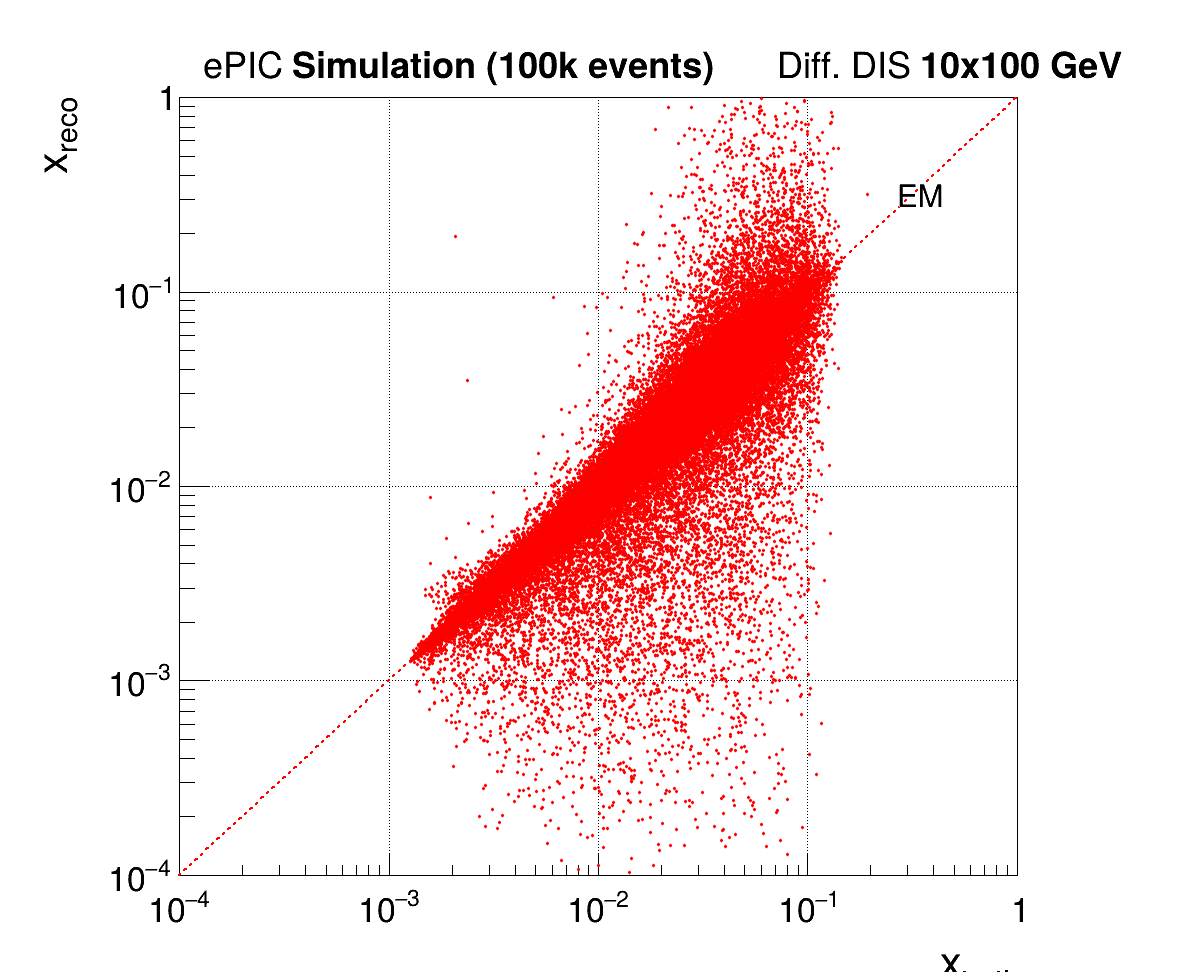
\includegraphics[width=\linewidth]{../figs/inclusive/histos/xbj_corr_unbinned_em.png}
    \column{0.25\textwidth}
    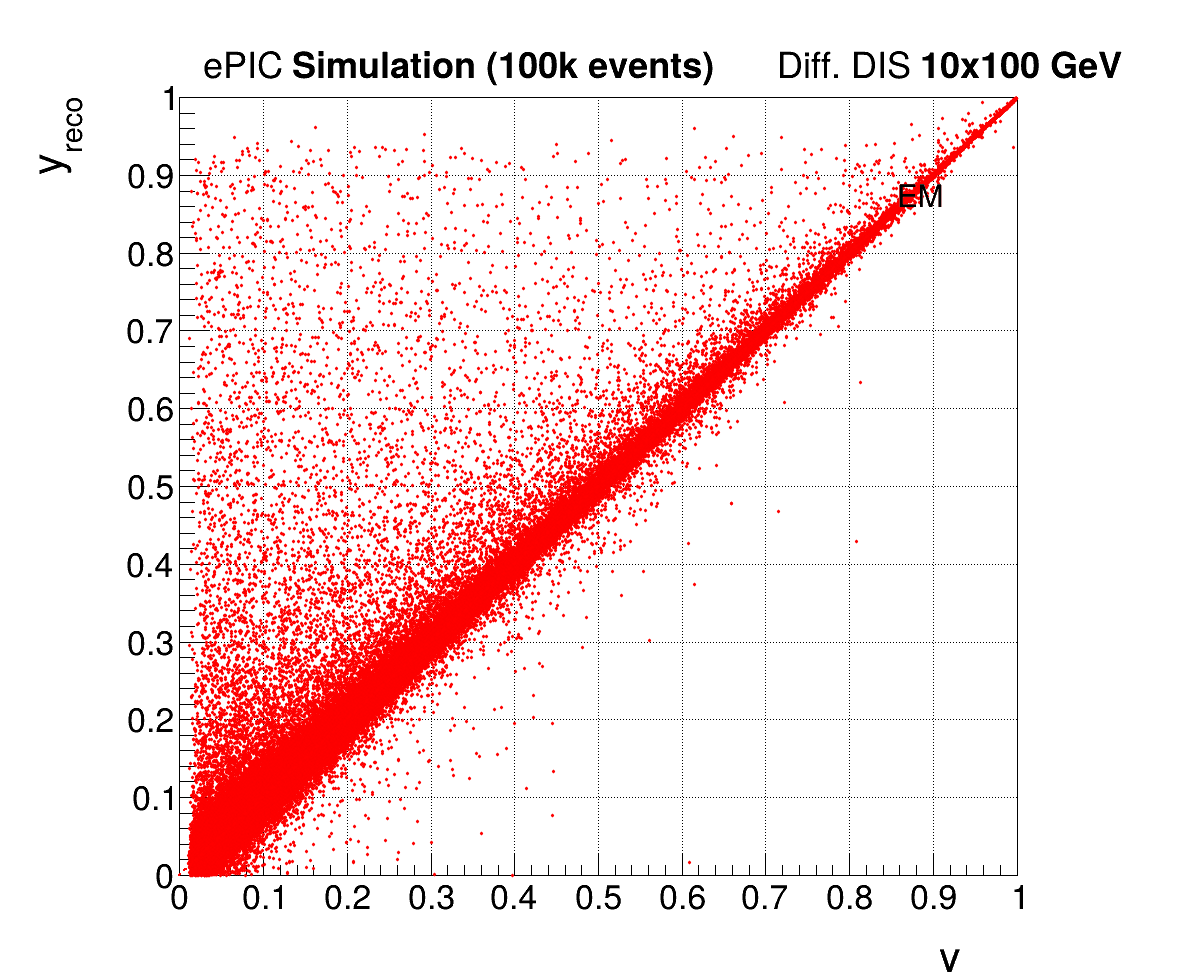
\includegraphics[width=\linewidth]{../figs/inclusive/histos/y_corr_unbinned_em.png}
    \vspace{0.2cm}
    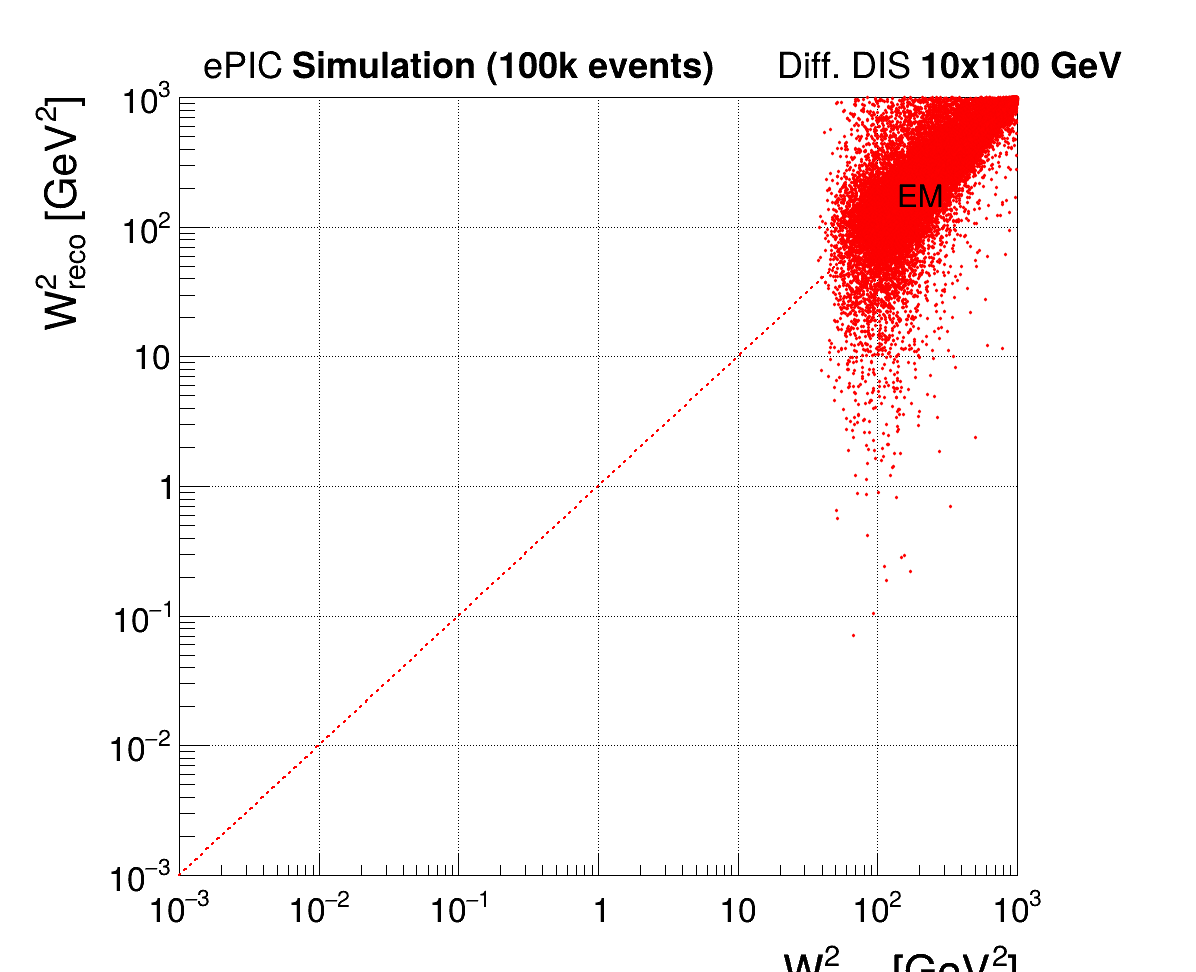
\includegraphics[width=\linewidth]{../figs/inclusive/histos/w2_corr_unbinned_em.png}
  \end{columns}
\end{frame}

\begin{frame}{Inclusive Resolutions}
  \begin{columns}
    \column{0.35\textwidth}
    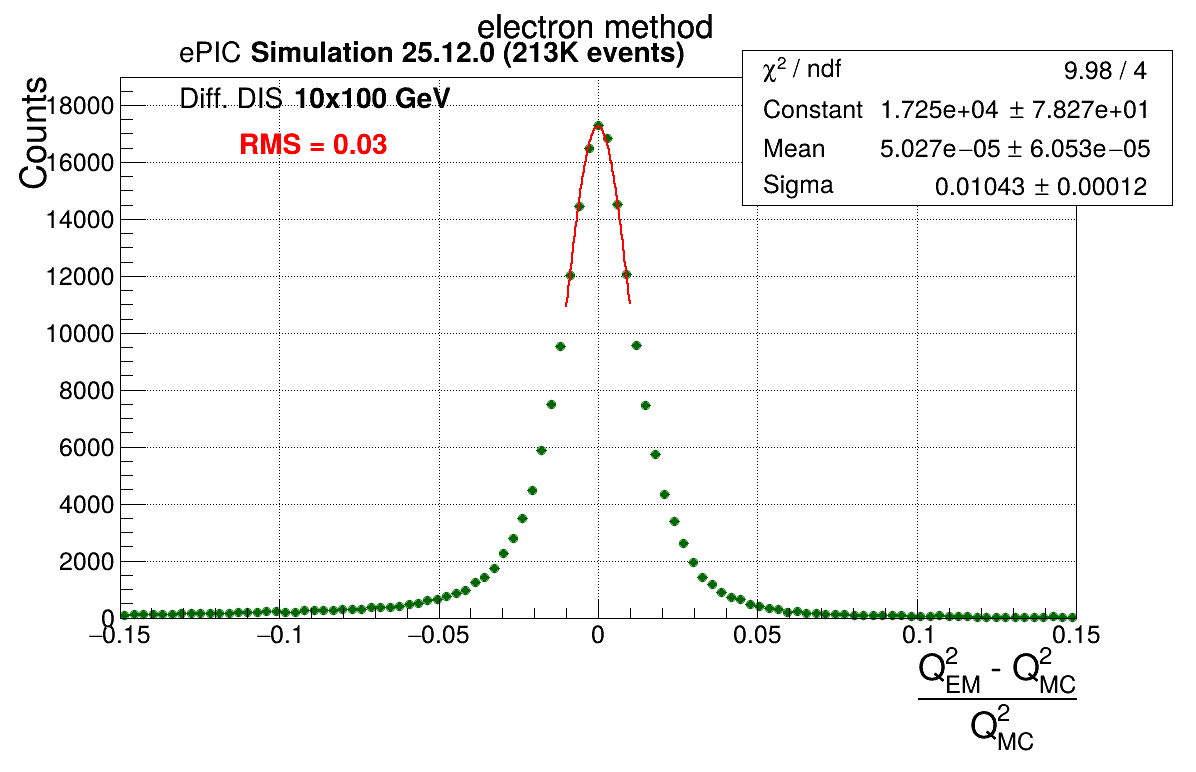
\includegraphics[width=\linewidth]{../figs/inclusive/resolution/q2_relres_em.png}
    \vspace{0.2cm}
    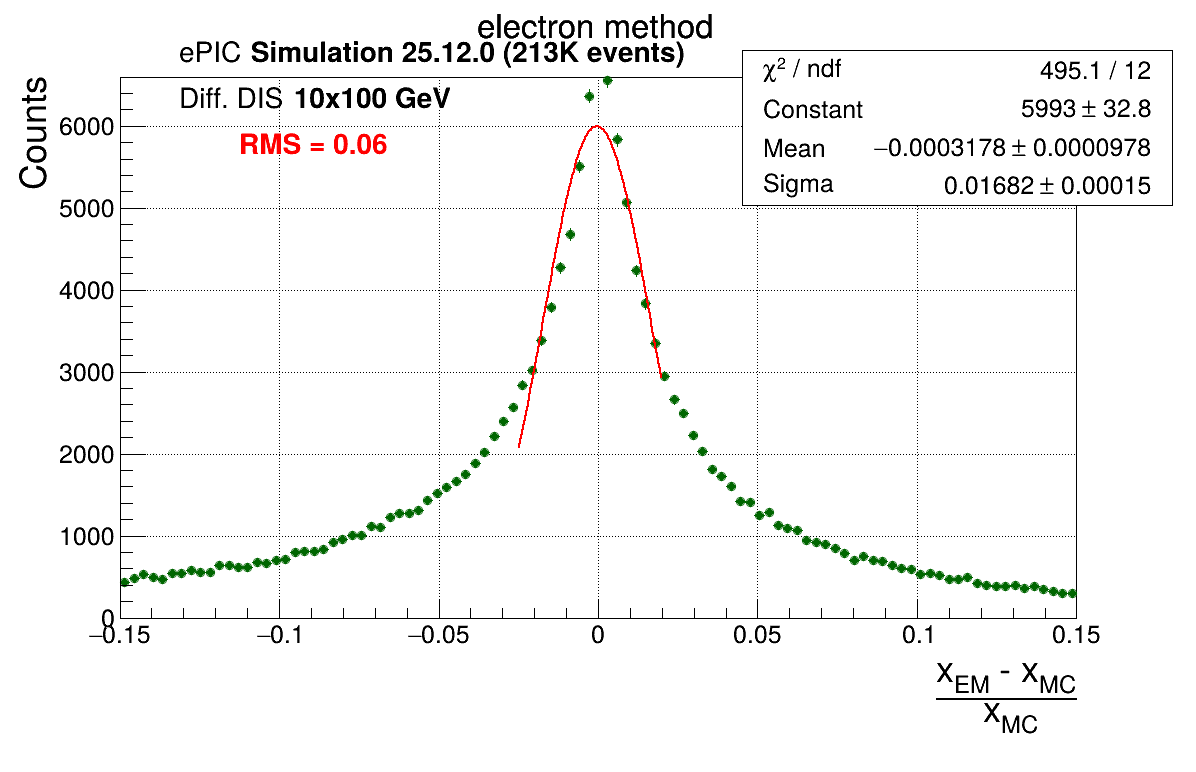
\includegraphics[width=\linewidth]{../figs/inclusive/resolution/xbj_relres_em.png}
    \column{0.35\textwidth}
    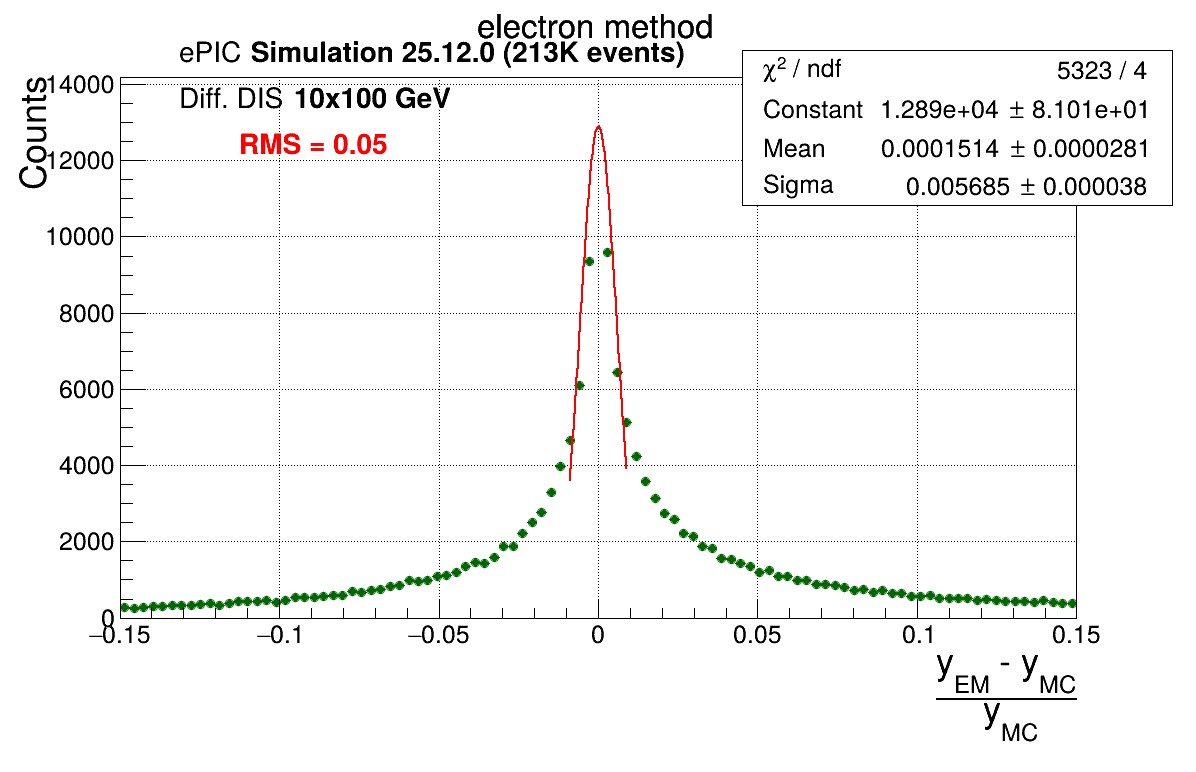
\includegraphics[width=\linewidth]{../figs/inclusive/resolution/y_relres_em.png}
    \vspace{0.2cm}
    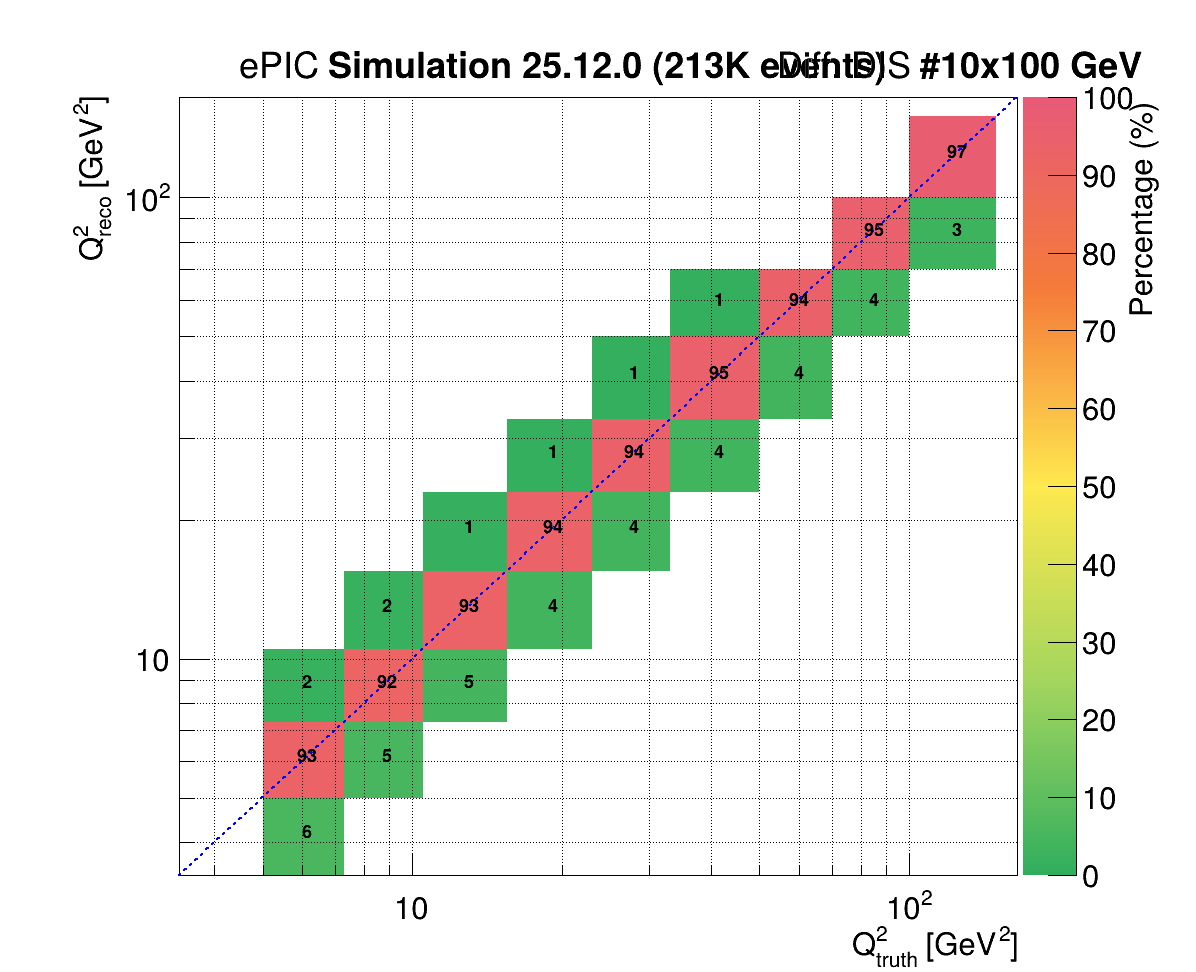
\includegraphics[width=\linewidth]{../figs/inclusive/response/response_q2_electron_raw.png}
  \end{columns}
\end{frame}

\begin{frame}{Diffractive |t|}
  \begin{columns}
    \column{0.35\textwidth}
    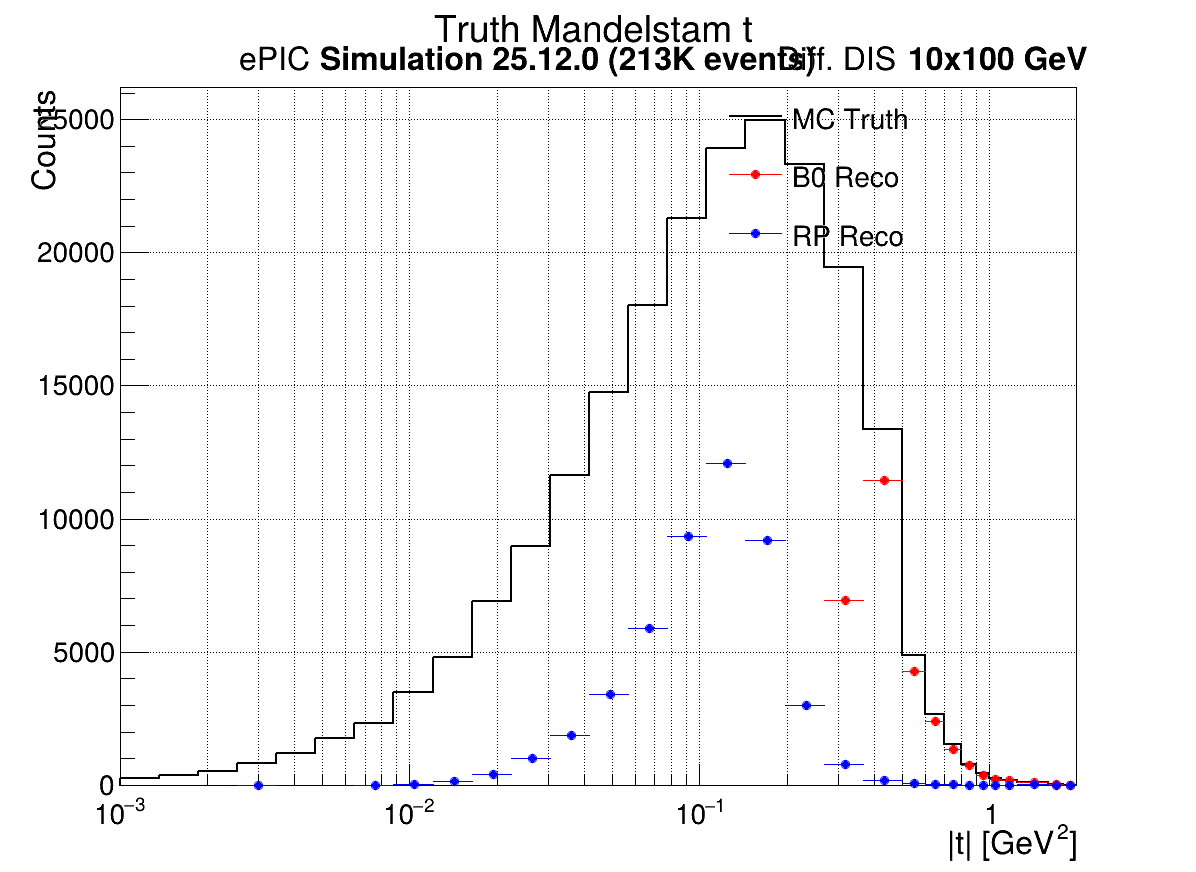
\includegraphics[width=\linewidth]{../figs/diffractive/histos/t_distributions.png}
    \vspace{0.2cm}
    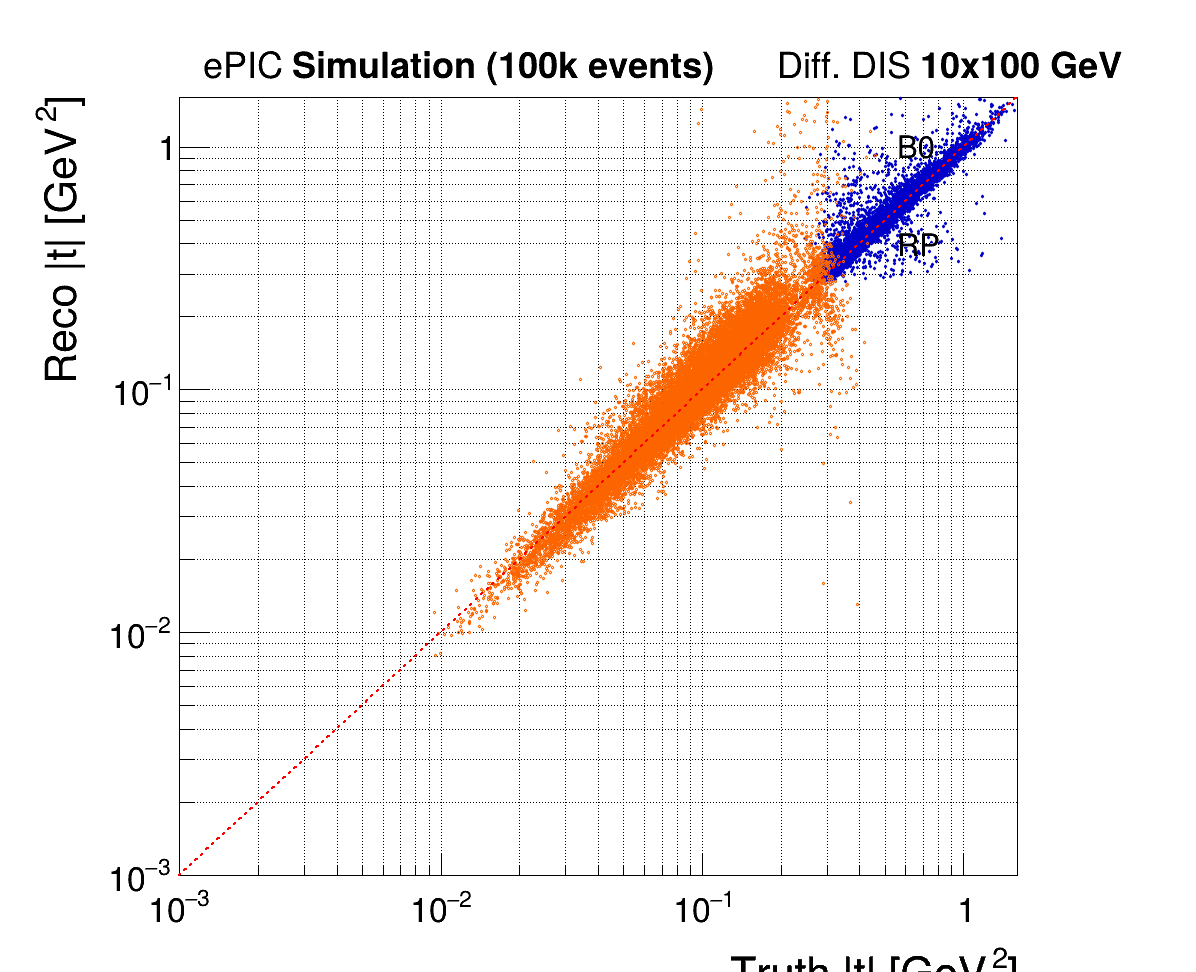
\includegraphics[width=\linewidth]{../figs/diffractive/histos/t_corr_unbinned.png}
    \column{0.35\textwidth}
    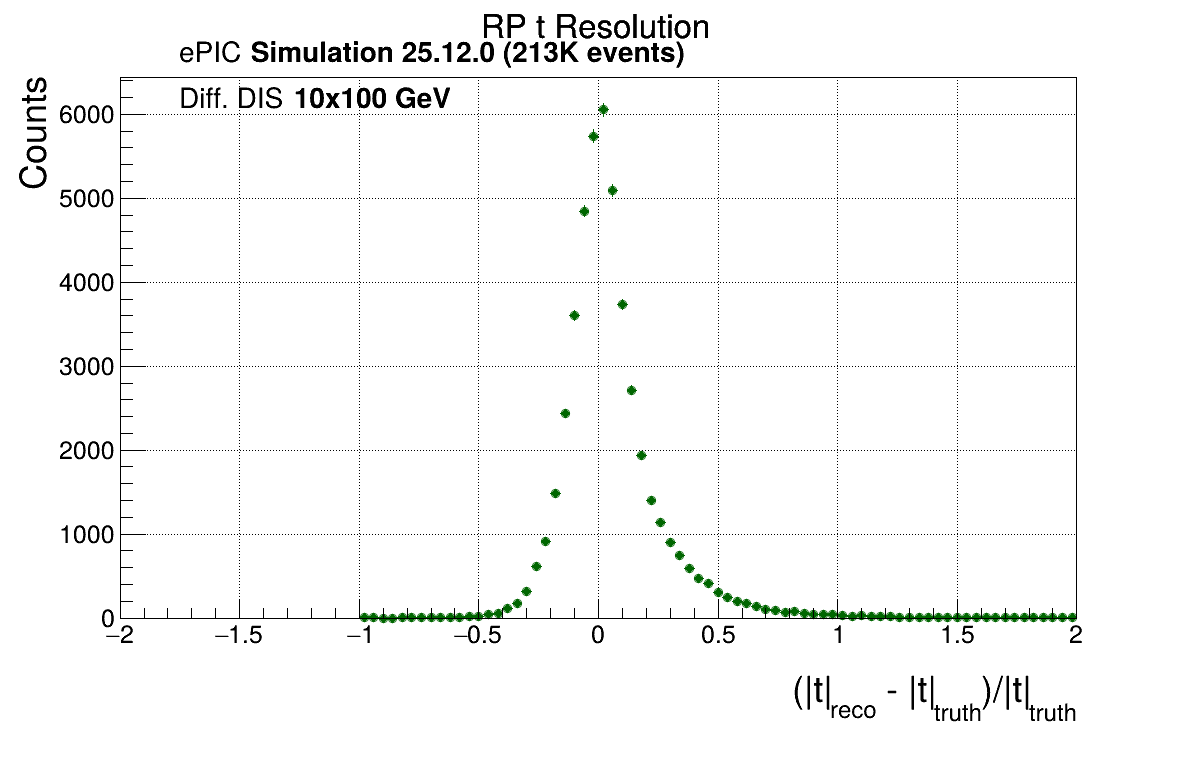
\includegraphics[width=\linewidth]{../figs/diffractive/resolution/t_res_rp.png}
 %   \vspace{0.2cm}
  %  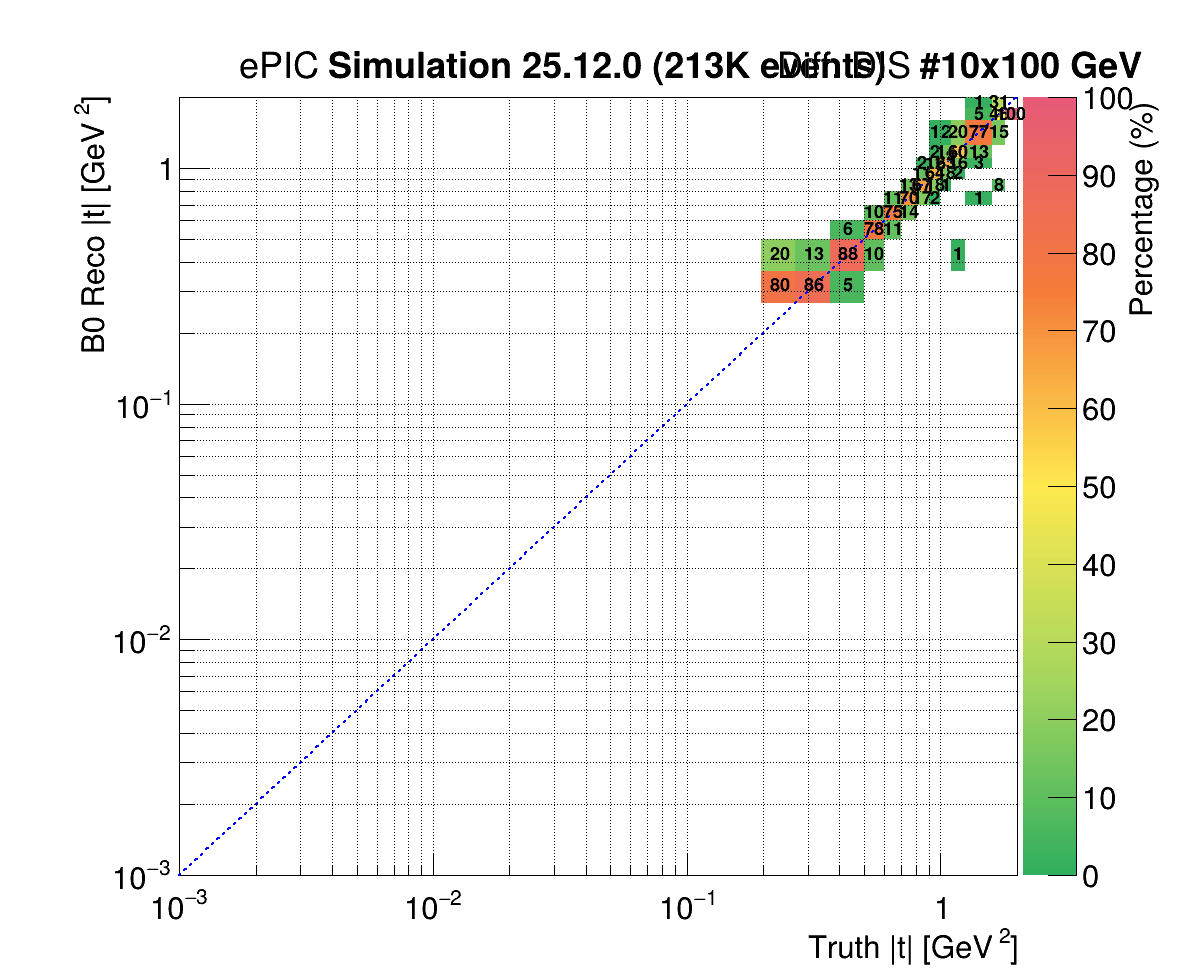
\includegraphics[width=\linewidth]{../figs/diffractive/response/response_t_b0.png}
  \end{columns}
\end{frame}

\begin{frame}{$x_L$ Observables}
  \begin{columns}
    \column{0.45\textwidth}
    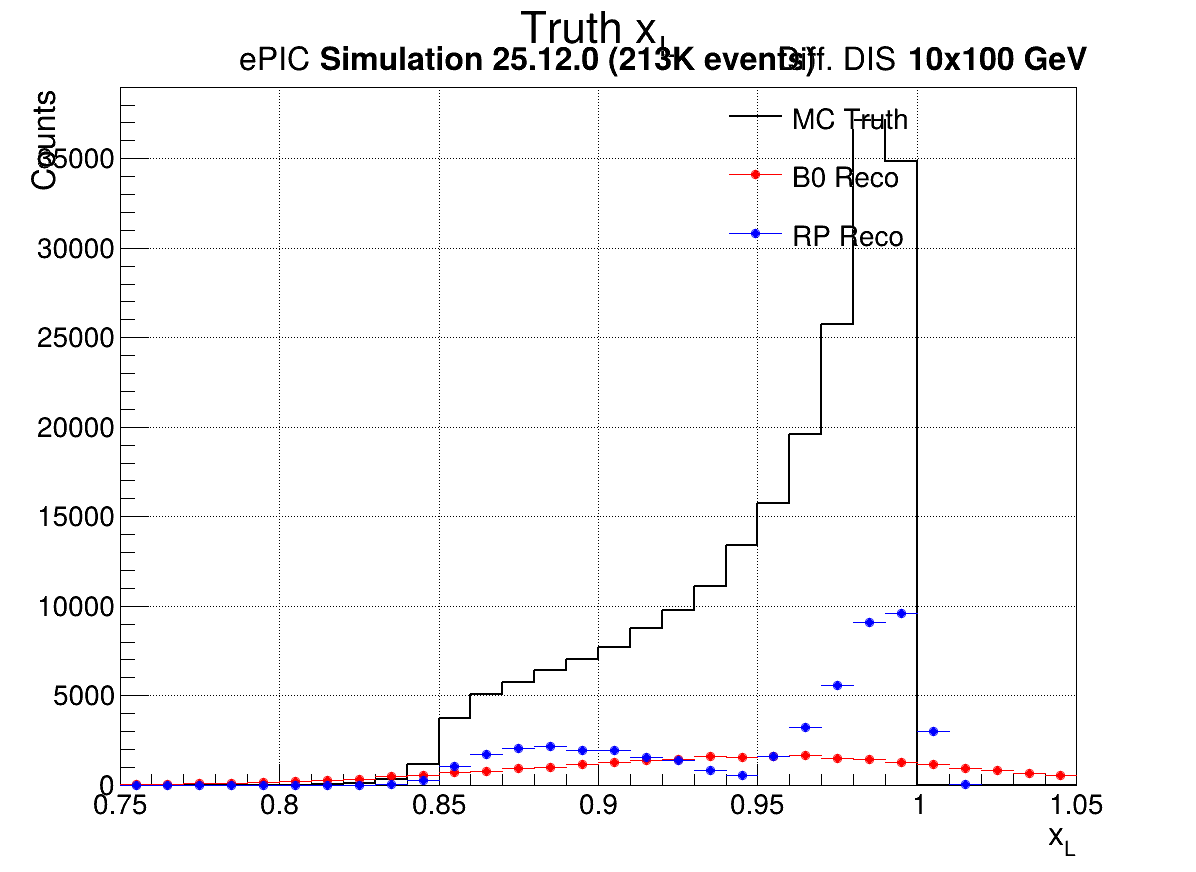
\includegraphics[width=\linewidth]{../figs/diffractive/histos/xL_distributions.png}
    \column{0.45\textwidth}
    \includegraphics[width=\linewidth]{../figs/diffractive/histos/xL_corr_unbinned.png}
  \end{columns}
\end{frame}

\begin{frame}{Next Steps}
  \begin{itemize}
    \item Rest of the plots $\beta, x_\mathrm{Pom}$, cross section
    \item Systematic checks and unfolding studies
    \item still filling the AN
    \item Shorten the AN
  \end{itemize}
\end{frame}

\end{document}
